% Options for packages loaded elsewhere
\PassOptionsToPackage{unicode}{hyperref}
\PassOptionsToPackage{hyphens}{url}
\PassOptionsToPackage{dvipsnames,svgnames,x11names}{xcolor}
%
\documentclass[
  letterpaper,
  DIV=11,
  numbers=noendperiod]{scrartcl}

\usepackage{amsmath,amssymb}
\usepackage{iftex}
\ifPDFTeX
  \usepackage[T1]{fontenc}
  \usepackage[utf8]{inputenc}
  \usepackage{textcomp} % provide euro and other symbols
\else % if luatex or xetex
  \usepackage{unicode-math}
  \defaultfontfeatures{Scale=MatchLowercase}
  \defaultfontfeatures[\rmfamily]{Ligatures=TeX,Scale=1}
\fi
\usepackage{lmodern}
\ifPDFTeX\else  
    % xetex/luatex font selection
\fi
% Use upquote if available, for straight quotes in verbatim environments
\IfFileExists{upquote.sty}{\usepackage{upquote}}{}
\IfFileExists{microtype.sty}{% use microtype if available
  \usepackage[]{microtype}
  \UseMicrotypeSet[protrusion]{basicmath} % disable protrusion for tt fonts
}{}
\makeatletter
\@ifundefined{KOMAClassName}{% if non-KOMA class
  \IfFileExists{parskip.sty}{%
    \usepackage{parskip}
  }{% else
    \setlength{\parindent}{0pt}
    \setlength{\parskip}{6pt plus 2pt minus 1pt}}
}{% if KOMA class
  \KOMAoptions{parskip=half}}
\makeatother
\usepackage{xcolor}
\setlength{\emergencystretch}{3em} % prevent overfull lines
\setcounter{secnumdepth}{5}
% Make \paragraph and \subparagraph free-standing
\ifx\paragraph\undefined\else
  \let\oldparagraph\paragraph
  \renewcommand{\paragraph}[1]{\oldparagraph{#1}\mbox{}}
\fi
\ifx\subparagraph\undefined\else
  \let\oldsubparagraph\subparagraph
  \renewcommand{\subparagraph}[1]{\oldsubparagraph{#1}\mbox{}}
\fi

\usepackage{color}
\usepackage{fancyvrb}
\newcommand{\VerbBar}{|}
\newcommand{\VERB}{\Verb[commandchars=\\\{\}]}
\DefineVerbatimEnvironment{Highlighting}{Verbatim}{commandchars=\\\{\}}
% Add ',fontsize=\small' for more characters per line
\usepackage{framed}
\definecolor{shadecolor}{RGB}{241,243,245}
\newenvironment{Shaded}{\begin{snugshade}}{\end{snugshade}}
\newcommand{\AlertTok}[1]{\textcolor[rgb]{0.68,0.00,0.00}{#1}}
\newcommand{\AnnotationTok}[1]{\textcolor[rgb]{0.37,0.37,0.37}{#1}}
\newcommand{\AttributeTok}[1]{\textcolor[rgb]{0.40,0.45,0.13}{#1}}
\newcommand{\BaseNTok}[1]{\textcolor[rgb]{0.68,0.00,0.00}{#1}}
\newcommand{\BuiltInTok}[1]{\textcolor[rgb]{0.00,0.23,0.31}{#1}}
\newcommand{\CharTok}[1]{\textcolor[rgb]{0.13,0.47,0.30}{#1}}
\newcommand{\CommentTok}[1]{\textcolor[rgb]{0.37,0.37,0.37}{#1}}
\newcommand{\CommentVarTok}[1]{\textcolor[rgb]{0.37,0.37,0.37}{\textit{#1}}}
\newcommand{\ConstantTok}[1]{\textcolor[rgb]{0.56,0.35,0.01}{#1}}
\newcommand{\ControlFlowTok}[1]{\textcolor[rgb]{0.00,0.23,0.31}{\textbf{#1}}}
\newcommand{\DataTypeTok}[1]{\textcolor[rgb]{0.68,0.00,0.00}{#1}}
\newcommand{\DecValTok}[1]{\textcolor[rgb]{0.68,0.00,0.00}{#1}}
\newcommand{\DocumentationTok}[1]{\textcolor[rgb]{0.37,0.37,0.37}{\textit{#1}}}
\newcommand{\ErrorTok}[1]{\textcolor[rgb]{0.68,0.00,0.00}{#1}}
\newcommand{\ExtensionTok}[1]{\textcolor[rgb]{0.00,0.23,0.31}{#1}}
\newcommand{\FloatTok}[1]{\textcolor[rgb]{0.68,0.00,0.00}{#1}}
\newcommand{\FunctionTok}[1]{\textcolor[rgb]{0.28,0.35,0.67}{#1}}
\newcommand{\ImportTok}[1]{\textcolor[rgb]{0.00,0.46,0.62}{#1}}
\newcommand{\InformationTok}[1]{\textcolor[rgb]{0.37,0.37,0.37}{#1}}
\newcommand{\KeywordTok}[1]{\textcolor[rgb]{0.00,0.23,0.31}{\textbf{#1}}}
\newcommand{\NormalTok}[1]{\textcolor[rgb]{0.00,0.23,0.31}{#1}}
\newcommand{\OperatorTok}[1]{\textcolor[rgb]{0.37,0.37,0.37}{#1}}
\newcommand{\OtherTok}[1]{\textcolor[rgb]{0.00,0.23,0.31}{#1}}
\newcommand{\PreprocessorTok}[1]{\textcolor[rgb]{0.68,0.00,0.00}{#1}}
\newcommand{\RegionMarkerTok}[1]{\textcolor[rgb]{0.00,0.23,0.31}{#1}}
\newcommand{\SpecialCharTok}[1]{\textcolor[rgb]{0.37,0.37,0.37}{#1}}
\newcommand{\SpecialStringTok}[1]{\textcolor[rgb]{0.13,0.47,0.30}{#1}}
\newcommand{\StringTok}[1]{\textcolor[rgb]{0.13,0.47,0.30}{#1}}
\newcommand{\VariableTok}[1]{\textcolor[rgb]{0.07,0.07,0.07}{#1}}
\newcommand{\VerbatimStringTok}[1]{\textcolor[rgb]{0.13,0.47,0.30}{#1}}
\newcommand{\WarningTok}[1]{\textcolor[rgb]{0.37,0.37,0.37}{\textit{#1}}}

\providecommand{\tightlist}{%
  \setlength{\itemsep}{0pt}\setlength{\parskip}{0pt}}\usepackage{longtable,booktabs,array}
\usepackage{calc} % for calculating minipage widths
% Correct order of tables after \paragraph or \subparagraph
\usepackage{etoolbox}
\makeatletter
\patchcmd\longtable{\par}{\if@noskipsec\mbox{}\fi\par}{}{}
\makeatother
% Allow footnotes in longtable head/foot
\IfFileExists{footnotehyper.sty}{\usepackage{footnotehyper}}{\usepackage{footnote}}
\makesavenoteenv{longtable}
\usepackage{graphicx}
\makeatletter
\def\maxwidth{\ifdim\Gin@nat@width>\linewidth\linewidth\else\Gin@nat@width\fi}
\def\maxheight{\ifdim\Gin@nat@height>\textheight\textheight\else\Gin@nat@height\fi}
\makeatother
% Scale images if necessary, so that they will not overflow the page
% margins by default, and it is still possible to overwrite the defaults
% using explicit options in \includegraphics[width, height, ...]{}
\setkeys{Gin}{width=\maxwidth,height=\maxheight,keepaspectratio}
% Set default figure placement to htbp
\makeatletter
\def\fps@figure{htbp}
\makeatother

\KOMAoption{captions}{tableheading}
\makeatletter
\@ifpackageloaded{caption}{}{\usepackage{caption}}
\AtBeginDocument{%
\ifdefined\contentsname
  \renewcommand*\contentsname{Table of contents}
\else
  \newcommand\contentsname{Table of contents}
\fi
\ifdefined\listfigurename
  \renewcommand*\listfigurename{List of Figures}
\else
  \newcommand\listfigurename{List of Figures}
\fi
\ifdefined\listtablename
  \renewcommand*\listtablename{List of Tables}
\else
  \newcommand\listtablename{List of Tables}
\fi
\ifdefined\figurename
  \renewcommand*\figurename{Figure}
\else
  \newcommand\figurename{Figure}
\fi
\ifdefined\tablename
  \renewcommand*\tablename{Table}
\else
  \newcommand\tablename{Table}
\fi
}
\@ifpackageloaded{float}{}{\usepackage{float}}
\floatstyle{ruled}
\@ifundefined{c@chapter}{\newfloat{codelisting}{h}{lop}}{\newfloat{codelisting}{h}{lop}[chapter]}
\floatname{codelisting}{Listing}
\newcommand*\listoflistings{\listof{codelisting}{List of Listings}}
\makeatother
\makeatletter
\makeatother
\makeatletter
\@ifpackageloaded{caption}{}{\usepackage{caption}}
\@ifpackageloaded{subcaption}{}{\usepackage{subcaption}}
\makeatother
\ifLuaTeX
  \usepackage{selnolig}  % disable illegal ligatures
\fi
\usepackage{bookmark}

\IfFileExists{xurl.sty}{\usepackage{xurl}}{} % add URL line breaks if available
\urlstyle{same} % disable monospaced font for URLs
\hypersetup{
  pdftitle={Churn Case},
  pdfauthor={Mette},
  colorlinks=true,
  linkcolor={blue},
  filecolor={Maroon},
  citecolor={Blue},
  urlcolor={Blue},
  pdfcreator={LaTeX via pandoc}}

\title{Churn Case}
\author{Mette}
\date{2024-03-07}

\begin{document}
\maketitle

\renewcommand*\contentsname{Table of contents}
{
\hypersetup{linkcolor=}
\setcounter{tocdepth}{3}
\tableofcontents
}
\begin{figure}[H]

{\centering 
\includegraphics{churnbillede.jpg}

}

\caption{Churn rates}

\end{figure}%

\section{Introduction}\label{introduction}

This case focuses on customer churn (also known as customer attrition or
customer turnover). Customer churn is interesting because it is usually
much cheaper to retain existing customers than to acquire new ones.
Instead of focusing on each individual customer, we will attempt to
build a predictive model that can help us decide which customers we
should focus our retention efforts on.

\section{Analysis}\label{analysis}

I follow the CRISP-DM (Cross-Industry Standard Process for Data Mining)
framework in my data mining projects, guiding me through six phases:
Business Understanding, Data Understanding, Data Preparation, Modeling,
Evaluation, and Deployment. This structured approach ensures I
effectively extract insights and apply data science.

\subsection{Business Understanding}\label{business-understanding}

Understanding customer churn is critical for banks as it aids in cost
reduction by prioritizing the retention of existing customers over
acquiring new ones. This not only helps in stabilizing revenue but also
enhances customer satisfaction by addressing their specific needs and
concerns. By gaining insights into churn patterns, banks can develop
targeted strategies, optimize resource allocation, and gain a
competitive edge in the market.

\subsection{Data Understanding}\label{data-understanding}

\subsubsection{Reading libraries}\label{reading-libraries}

We will start by loading the nessescary libraries

\begin{Shaded}
\begin{Highlighting}[]
\NormalTok{pacman}\SpecialCharTok{::}\FunctionTok{p\_load}\NormalTok{(}\StringTok{"tidyverse"}\NormalTok{, }\StringTok{"magrittr"}\NormalTok{, }\StringTok{"nycflights13"}\NormalTok{, }\StringTok{"gapminder"}\NormalTok{,}
               \StringTok{"Lahman"}\NormalTok{, }\StringTok{"maps"}\NormalTok{, }\StringTok{"lubridate"}\NormalTok{, }\StringTok{"pryr"}\NormalTok{, }\StringTok{"hms"}\NormalTok{, }\StringTok{"hexbin"}\NormalTok{,}
               \StringTok{"feather"}\NormalTok{, }\StringTok{"htmlwidgets"}\NormalTok{, }\StringTok{"broom"}\NormalTok{, }\StringTok{"pander"}\NormalTok{, }\StringTok{"modelr"}\NormalTok{,}
               \StringTok{"XML"}\NormalTok{, }\StringTok{"httr"}\NormalTok{, }\StringTok{"jsonlite"}\NormalTok{, }\StringTok{"lubridate"}\NormalTok{, }\StringTok{"microbenchmark"}\NormalTok{,}
               \StringTok{"splines"}\NormalTok{, }\StringTok{"ISLR2"}\NormalTok{, }\StringTok{"MASS"}\NormalTok{, }\StringTok{"testthat"}\NormalTok{,  }\StringTok{"caret"}\NormalTok{,}
               \StringTok{"RSQLite"}\NormalTok{, }\StringTok{"class"}\NormalTok{, }\StringTok{"babynames"}\NormalTok{, }\StringTok{"nasaweather"}\NormalTok{, }\StringTok{"pls"}\NormalTok{,}
               \StringTok{"fueleconomy"}\NormalTok{, }\StringTok{"viridis"}\NormalTok{, }\StringTok{"boot"}\NormalTok{, }\StringTok{"devtools"}\NormalTok{, }\StringTok{"tree"}\NormalTok{, }\StringTok{"leaps"}\NormalTok{,}
               \StringTok{"glmnet"}\NormalTok{, }\StringTok{"gam"}\NormalTok{, }\StringTok{"akima"}\NormalTok{, }\StringTok{"factoextra"}\NormalTok{, }\StringTok{"randomForest"}\NormalTok{, }\StringTok{"gbm"}\NormalTok{, }
               \StringTok{"ggrepel"}\NormalTok{, }\StringTok{"GGally"}\NormalTok{, }\StringTok{"fmsb"}\NormalTok{, }\StringTok{"sjPlot"}\NormalTok{, }\StringTok{"rcompanion"}\NormalTok{, }\StringTok{"DT"}\NormalTok{)}
\end{Highlighting}
\end{Shaded}

\subsubsection{Importing data}\label{importing-data}

The dataset we are going to work with will be imported and investigated.

\begin{Shaded}
\begin{Highlighting}[]
\CommentTok{\#bank\_churn \textless{}{-} read.csv("Churn\_Modelling.csv")}
\NormalTok{bank\_churn }\OtherTok{\textless{}{-}} \FunctionTok{read.csv}\NormalTok{(}\StringTok{"C:/Users/mette/OneDrive/Skrivebord/PB dataanalyse/Programmering og statistical learning/data/Portfolio/Churn\_Modelling.csv"}\NormalTok{)}


\CommentTok{\#tjekker data og klasser}
\FunctionTok{str}\NormalTok{(bank\_churn)}
\end{Highlighting}
\end{Shaded}

\begin{Shaded}
\begin{Highlighting}[]
\CommentTok{\#vi skaber en interaktiv tabel}

\FunctionTok{datatable}\NormalTok{(bank\_churn, }\AttributeTok{caption =}\NormalTok{ htmltools}\SpecialCharTok{::}\NormalTok{tags}\SpecialCharTok{$}\FunctionTok{caption}\NormalTok{(}
    \AttributeTok{style =} \StringTok{\textquotesingle{}caption{-}side: top; text{-}align: center;\textquotesingle{}}\NormalTok{,}
    \StringTok{\textquotesingle{}Table 1: \textquotesingle{}}\NormalTok{, htmltools}\SpecialCharTok{::}\FunctionTok{em}\NormalTok{(}\StringTok{\textquotesingle{}Bank data \textquotesingle{}}\NormalTok{))}
\NormalTok{    )}
\end{Highlighting}
\end{Shaded}

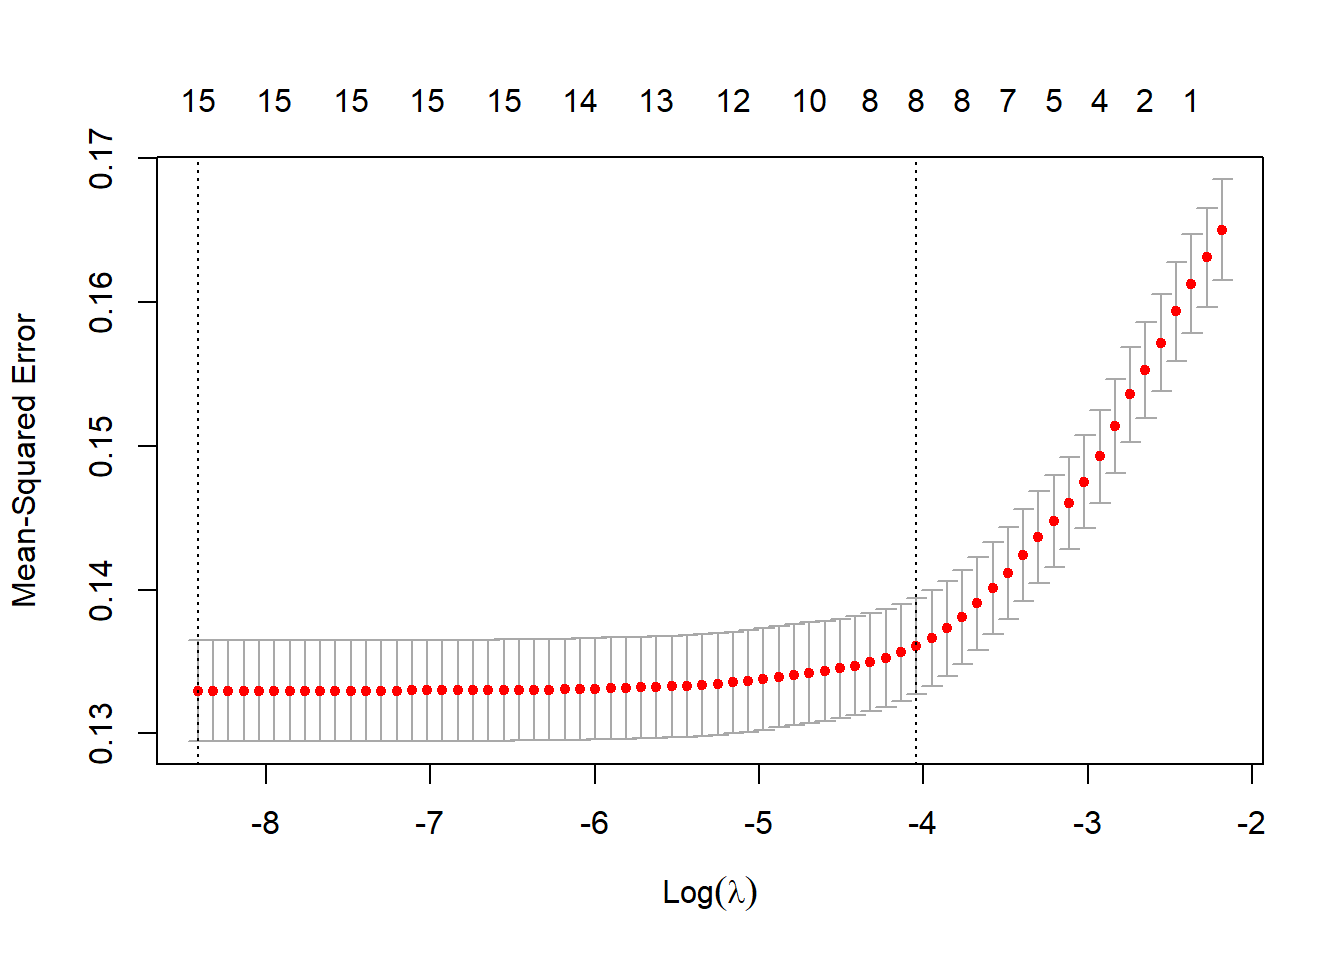
\includegraphics{index_files/figure-pdf/unnamed-chunk-3-1.pdf}

\subsection{Data Preparation}\label{data-preparation}

\subsubsection{Cleaning data}\label{cleaning-data}

First we are checking for missing values. There are no missing values in
the TotalCharges variable. We are imputing thesevalues with the
meanvalue, since the quantity is low. After this we are changes all the
character class variables to factors for later statistical analysis. The
data is normalised and finally the churndataset is again changes to a
dataframe and the CustomerID variable is removed.

\begin{Shaded}
\begin{Highlighting}[]
\CommentTok{\# Beregn antallet af missing værdier i hver kolonne. No missing}
\NormalTok{bank\_churn }\SpecialCharTok{\%\textgreater{}\%}\NormalTok{ purrr}\SpecialCharTok{::}\FunctionTok{map}\NormalTok{(}\SpecialCharTok{\textasciitilde{}} \FunctionTok{sum}\NormalTok{(}\FunctionTok{is.na}\NormalTok{(.)))}

\FunctionTok{summary}\NormalTok{(bank\_churn)}

\CommentTok{\# There are no missin values, so we can proceed.}

\CommentTok{\#the relevant variables are converted into factors.}

\CommentTok{\# Type = factor and integers{-}{-}{-}{-}{-}{-}{-}{-}{-}{-}{-}{-}{-}{-}{-}{-}{-}{-}{-}{-}{-}{-}{-}{-}{-}{-}{-}{-}{-}{-}{-}{-}{-}{-}{-}{-}{-}{-}{-}{-}{-}{-}{-}{-}{-}{-}{-}{-}{-}{-}{-}{-}{-}{-}{-}{-}{-}{-}{-}}

\NormalTok{bank\_churn\_fact }\OtherTok{\textless{}{-}}\NormalTok{ bank\_churn }\SpecialCharTok{\%\textgreater{}\%}
  \FunctionTok{mutate\_if}\NormalTok{(is.character, as.factor) }\SpecialCharTok{\%\textgreater{}\%}
  \FunctionTok{mutate\_if}\NormalTok{(is.integer, as.factor)}

\NormalTok{bank\_churn\_fact}\SpecialCharTok{$}\NormalTok{CreditScore }\OtherTok{\textless{}{-}} \FunctionTok{as.integer}\NormalTok{(bank\_churn\_fact}\SpecialCharTok{$}\NormalTok{CreditScore)}
\NormalTok{bank\_churn\_fact}\SpecialCharTok{$}\NormalTok{Age }\OtherTok{\textless{}{-}} \FunctionTok{as.integer}\NormalTok{(bank\_churn\_fact}\SpecialCharTok{$}\NormalTok{Age)}
\NormalTok{bank\_churn\_fact}\SpecialCharTok{$}\NormalTok{Tenure }\OtherTok{\textless{}{-}} \FunctionTok{as.integer}\NormalTok{(bank\_churn\_fact}\SpecialCharTok{$}\NormalTok{Tenure)}
\FunctionTok{str}\NormalTok{(bank\_churn\_fact)}

\CommentTok{\# Normalisering {-}{-}{-}{-}{-}{-}{-}{-}{-}{-}{-}{-}{-}{-}{-}{-}{-}{-}{-}{-}{-}{-}{-}{-}{-}{-}{-}{-}{-}{-}{-}{-}{-}{-}{-}{-}{-}{-}{-}{-}{-}{-}{-}{-}{-}{-}{-}{-}{-}{-}{-}{-}{-}{-}{-}{-}{-}{-}{-}}

\CommentTok{\# Det er ikke nødvendigt at normalisere data i forbindelse med de statistiske}
\CommentTok{\# modeller, som vi skal køre her. Der er forskellige typer af normalisering. }
\CommentTok{\# Vi ser her på følgende:}

\NormalTok{normalize }\OtherTok{\textless{}{-}} \ControlFlowTok{function}\NormalTok{(x) \{}
\NormalTok{  ((x}\SpecialCharTok{{-}}\FunctionTok{min}\NormalTok{(x))}\SpecialCharTok{/}\NormalTok{(}\FunctionTok{max}\NormalTok{(x)}\SpecialCharTok{{-}}\FunctionTok{min}\NormalTok{(x)))}
\NormalTok{\}}

\NormalTok{bank\_churn\_fact }\OtherTok{\textless{}{-}}\NormalTok{ bank\_churn\_fact }\SpecialCharTok{\%\textgreater{}\%} 
  \FunctionTok{mutate\_if}\NormalTok{(is.numeric, normalize)}

\NormalTok{bank\_churn\_fact }\OtherTok{\textless{}{-}}\NormalTok{ bank\_churn\_fact }\SpecialCharTok{\%\textgreater{}\%}
\NormalTok{  dplyr}\SpecialCharTok{::}\FunctionTok{select}\NormalTok{(Exited, }\FunctionTok{everything}\NormalTok{())}

\FunctionTok{glimpse}\NormalTok{(bank\_churn\_fact)}

\NormalTok{numeric\_columns }\OtherTok{\textless{}{-}} \FunctionTok{sapply}\NormalTok{(bank\_churn\_fact, is.numeric)}

\CommentTok{\# Konverter numeriske variable fra dbl til int}
\CommentTok{\#bank\_churn\_fact[numeric\_columns] \textless{}{-} lapply(bank\_churn\_fact[numeric\_columns], as.integer)}

\CommentTok{\# Fravalg af customerID, Efternavn og ID {-}{-}{-}{-}{-}{-}{-}{-}{-}{-}{-}{-}{-}{-}{-}{-}{-}{-}{-}{-}{-}{-}{-}{-}{-}{-}{-}{-}{-}{-}{-}{-}{-}{-}{-}{-}{-}{-}{-}{-}{-}{-}{-}{-}{-}{-}{-}{-}{-}{-}{-}}

\NormalTok{bank\_churn\_fact }\OtherTok{\textless{}{-}}\NormalTok{ bank\_churn\_fact }\SpecialCharTok{\%\textgreater{}\%} 
\NormalTok{  dplyr}\SpecialCharTok{::}\FunctionTok{select}\NormalTok{(}\SpecialCharTok{{-}}\NormalTok{RowNumber, }\SpecialCharTok{{-}}\NormalTok{CustomerId, }\SpecialCharTok{{-}}\NormalTok{Surname)}

\FunctionTok{names}\NormalTok{(bank\_churn\_fact)}

\CommentTok{\#Ændre variablen Exited til Churn}

\NormalTok{bank\_churn\_fact }\OtherTok{\textless{}{-}}\NormalTok{ bank\_churn\_fact }\SpecialCharTok{\%\textgreater{}\%}
  \FunctionTok{rename}\NormalTok{(}\AttributeTok{Churn =}\NormalTok{ Exited)}

\NormalTok{bank\_churn\_fact}\SpecialCharTok{$}\NormalTok{Churn }\OtherTok{\textless{}{-}} \FunctionTok{ifelse}\NormalTok{(bank\_churn\_fact}\SpecialCharTok{$}\NormalTok{Churn }\SpecialCharTok{==} \DecValTok{1}\NormalTok{, }\StringTok{"Yes"}\NormalTok{, }\StringTok{"No"}\NormalTok{)}
\NormalTok{bank\_churn\_fact}\SpecialCharTok{$}\NormalTok{Churn }\OtherTok{\textless{}{-}} \FunctionTok{as.factor}\NormalTok{(bank\_churn\_fact}\SpecialCharTok{$}\NormalTok{Churn)}
\FunctionTok{str}\NormalTok{((bank\_churn\_fact))}
\end{Highlighting}
\end{Shaded}

This creates a dataset with 10.000 observations, that can be
investigated and is ready for analysis.

\begin{Shaded}
\begin{Highlighting}[]
\CommentTok{\# Install DT package}
\FunctionTok{install.packages}\NormalTok{(}\StringTok{"DT"}\NormalTok{)}

\CommentTok{\# Load DT package}
\FunctionTok{library}\NormalTok{(DT)}

\FunctionTok{library}\NormalTok{(DT)}

\FunctionTok{datatable}\NormalTok{(bank\_churn\_fact, }
          \AttributeTok{options =} \FunctionTok{list}\NormalTok{(}\AttributeTok{pageLength =} \DecValTok{5}\NormalTok{, }\AttributeTok{autoWidth =} \ConstantTok{TRUE}\NormalTok{), }
          \AttributeTok{caption =} \StringTok{\textquotesingle{}Table 1: Telecommunication data\textquotesingle{}}\NormalTok{)}
\end{Highlighting}
\end{Shaded}

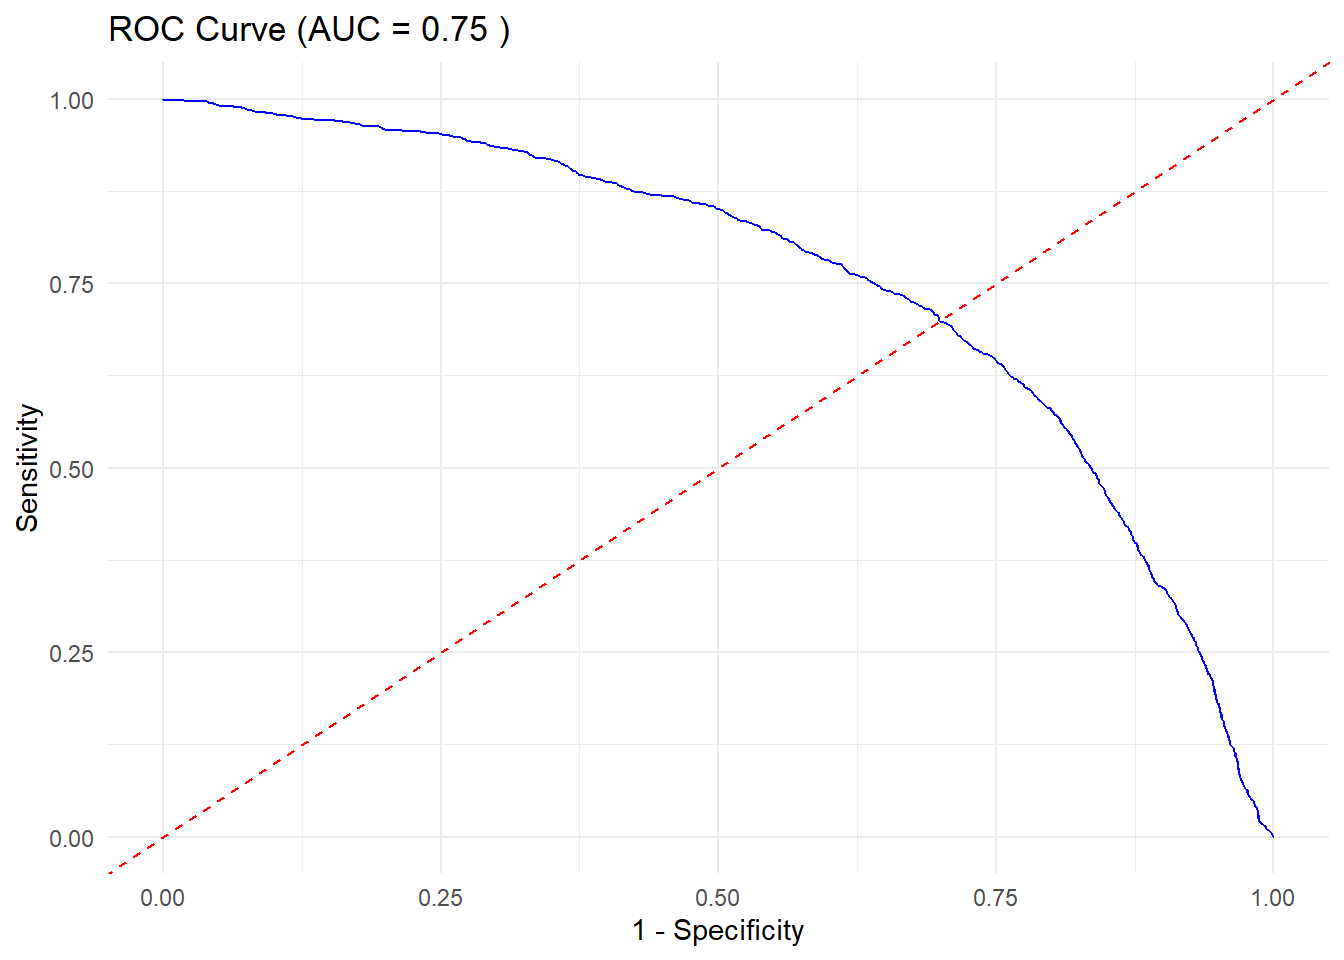
\includegraphics{index_files/figure-pdf/unnamed-chunk-5-1.pdf}

\subsection{Modeling}\label{modeling}

Training and test data

\begin{Shaded}
\begin{Highlighting}[]
\CommentTok{\#træningsdata og testdata}


\CommentTok{\# Vi bruger funktionen set.seed, så vi kan reproducere vores resultater}
\FunctionTok{set.seed}\NormalTok{(}\DecValTok{5}\NormalTok{)}
\CommentTok{\# træningsdel og testdel:}
\NormalTok{intrain }\OtherTok{\textless{}{-}} \FunctionTok{createDataPartition}\NormalTok{(}\AttributeTok{y=}\NormalTok{bank\_churn\_fact}\SpecialCharTok{$}\NormalTok{Churn,}
                               \AttributeTok{p=}\FloatTok{0.80}\NormalTok{, }\AttributeTok{list=}\ConstantTok{FALSE}\NormalTok{)}

\CommentTok{\# list=FALSE betyder at outputtet bliver en matrix og denne kan bruges }
\CommentTok{\# i koden nedenfor:}

\NormalTok{train }\OtherTok{\textless{}{-}}\NormalTok{ bank\_churn\_fact[intrain,]}
\NormalTok{test }\OtherTok{\textless{}{-}}\NormalTok{ bank\_churn\_fact[}\SpecialCharTok{{-}}\NormalTok{intrain,]}
\end{Highlighting}
\end{Shaded}

\subsubsection{\texorpdfstring{\textbf{Cost
Assessment}}{Cost Assessment}}\label{cost-assessment}

The cost assessment is significant when deciding on the threshold in
connection with, for example, logistic regression. The relative cost of
the different errors that can be made affects where it is optimal to
place the threshold. Optimal in terms of reducing costs. When we do not
have any a priori knowledge about the relative costs, we use a 50/50
split. But in this example, the situation is different. It does not cost
the same to commit the different errors.

\begin{Shaded}
\begin{Highlighting}[]
\CommentTok{\#                       |  Vil churne  | vil ikke churne}
\CommentTok{\# predikte churne       |      TP      |      FP}
\CommentTok{\# predikte ikke churne  |      FN      |      TN}
\end{Highlighting}
\end{Shaded}

Customer acquisition \$200
\href{https://www.reviewtrackers.com/blog/customer-acquisition-banking/\#:~:text=How\%20much\%20does\%20it\%20cost\%20a\%20bank\%20to,\%2866\%25\%29\%2C\%20and\%20SEO\%20\%2F\%20pay-per-click\%20\%28PPC\%29\%20advertising\%20\%2865\%25\%29.}{Se
documentation here})\{.uri\} - the cost for a false negative (FN)
prediction That is, predicting that a customer is satisfied when in
reality they churn. Customer retention \$40 (Source: Bain \& Company,
``The Value of Online Customer Loyalty in Retail Banking,'' 2016.) - the
cost of a false positive (FP) That is, predicting that a customer will
churn when in reality the customer was satisfied, and a true positive
(TP) that is, correctly predicting dissatisfied customers. Correctly
predicted true negatives (TN) cost nothing. That is, correctly
predicting that a customer is satisfied.

The situation until now is that the company assumes that no customers
churn. Thus the model is that nobody churns. In other words, the company
predicts a NO for every customer in the test dataset ,i.e., TP=FP=0. We
only need to calculate FN (since TN does not cost anything) ourselves.

The total savings from the new model based on a customer base of 10.000
customers:

\begin{Shaded}
\begin{Highlighting}[]
\NormalTok{FN\_omk }\OtherTok{\textless{}{-}} \DecValTok{200} 

\NormalTok{TP\_omk }\OtherTok{\textless{}{-}} \DecValTok{40}

\NormalTok{ FP\_omk }\OtherTok{\textless{}{-}}\NormalTok{ TP\_omk}

\NormalTok{ TN\_omk }\OtherTok{\textless{}{-}} \DecValTok{0}
\end{Highlighting}
\end{Shaded}

Calculation of the current model's costs based on the above information.
Since TN is free, we only need to calculate FN on the test dataset.
Remember, that all are expected not to churn, but a certain portion will
churn.

\begin{Shaded}
\begin{Highlighting}[]
\NormalTok{test}\SpecialCharTok{$}\NormalTok{no\_churn }\OtherTok{\textless{}{-}} \StringTok{"No"}
\NormalTok{FN\_simple }\OtherTok{\textless{}{-}} \FunctionTok{table}\NormalTok{(test}\SpecialCharTok{$}\NormalTok{Churn, test}\SpecialCharTok{$}\NormalTok{no\_churn)[}\DecValTok{2}\NormalTok{]}\SpecialCharTok{/}\NormalTok{(}\FunctionTok{table}\NormalTok{(test}\SpecialCharTok{$}\NormalTok{Churn, test}\SpecialCharTok{$}\NormalTok{no\_churn)[}\DecValTok{1}\NormalTok{]}\SpecialCharTok{+}
                                                    \FunctionTok{table}\NormalTok{(test}\SpecialCharTok{$}\NormalTok{Churn, test}\SpecialCharTok{$}\NormalTok{no\_churn)[}\DecValTok{2}\NormalTok{])}

\NormalTok{omkostninger\_mavefornemmelse }\OtherTok{\textless{}{-}}\NormalTok{ FN\_omk}\SpecialCharTok{*}\NormalTok{FN\_simple }\CommentTok{\# per kunde}


\NormalTok{test }\OtherTok{\textless{}{-}}\NormalTok{ dplyr}\SpecialCharTok{::}\FunctionTok{select}\NormalTok{(test, }\SpecialCharTok{{-}}\NormalTok{no\_churn) }\CommentTok{\# We dont need no churn anymore.}
\end{Highlighting}
\end{Shaded}

In order to evalutate the relevant variables we will perform Lasso
modelling

\begin{Shaded}
\begin{Highlighting}[]
\NormalTok{bank\_churn\_lasso }\OtherTok{\textless{}{-}}\NormalTok{ bank\_churn}

\NormalTok{bank\_churn\_lasso }\OtherTok{\textless{}{-}}\NormalTok{ bank\_churn\_lasso }\SpecialCharTok{\%\textgreater{}\%} 
\NormalTok{  dplyr}\SpecialCharTok{::}\FunctionTok{select}\NormalTok{(}\SpecialCharTok{{-}}\NormalTok{RowNumber, }\SpecialCharTok{{-}}\NormalTok{CustomerId, }\SpecialCharTok{{-}}\NormalTok{Surname)}

\FunctionTok{names}\NormalTok{(bank\_churn\_fact)}

\CommentTok{\#Ændre variablen Exited til Churn}

\NormalTok{bank\_churn\_lasso }\OtherTok{\textless{}{-}}\NormalTok{ bank\_churn\_lasso }\SpecialCharTok{\%\textgreater{}\%}
\NormalTok{  dplyr}\SpecialCharTok{::}\FunctionTok{rename}\NormalTok{(}\AttributeTok{Churn =}\NormalTok{ Exited)}



\FunctionTok{str}\NormalTok{(bank\_churn\_lasso)}


\NormalTok{x }\OtherTok{\textless{}{-}} \FunctionTok{model.matrix}\NormalTok{(Churn }\SpecialCharTok{\textasciitilde{}}\NormalTok{ ., bank\_churn\_lasso)[, }\SpecialCharTok{{-}}\DecValTok{1}\NormalTok{]}
\NormalTok{y }\OtherTok{\textless{}{-}}\NormalTok{ bank\_churn\_lasso}\SpecialCharTok{$}\NormalTok{Churn}

\NormalTok{grid }\OtherTok{\textless{}{-}} \DecValTok{10}\SpecialCharTok{\^{}}\FunctionTok{seq}\NormalTok{(}\DecValTok{10}\NormalTok{, }\SpecialCharTok{{-}}\DecValTok{2}\NormalTok{, }\AttributeTok{length =} \DecValTok{100}\NormalTok{)}
\NormalTok{lasso.mod }\OtherTok{\textless{}{-}} \FunctionTok{glmnet}\NormalTok{(x, y, }\AttributeTok{alpha =} \DecValTok{1}\NormalTok{, }\AttributeTok{lambda =}\NormalTok{ grid)}

\FunctionTok{coef}\NormalTok{(lasso.mod)}
\FunctionTok{dim}\NormalTok{(}\FunctionTok{coef}\NormalTok{(lasso.mod))}

\FunctionTok{names}\NormalTok{(bank\_churn\_lasso)}

\FunctionTok{set.seed}\NormalTok{(}\DecValTok{5}\NormalTok{)}
\NormalTok{train }\OtherTok{\textless{}{-}} \FunctionTok{sample}\NormalTok{(}\DecValTok{1}\SpecialCharTok{:}\FunctionTok{nrow}\NormalTok{(x), }\FunctionTok{nrow}\NormalTok{(x)}\SpecialCharTok{*}\DecValTok{2}\SpecialCharTok{/}\DecValTok{3}\NormalTok{)}
\NormalTok{test }\OtherTok{\textless{}{-}}\NormalTok{ (}\SpecialCharTok{{-}}\NormalTok{train)}
\NormalTok{y.test }\OtherTok{\textless{}{-}}\NormalTok{ y[test]}


\FunctionTok{set.seed}\NormalTok{(}\DecValTok{5}\NormalTok{)}
\NormalTok{cv.out }\OtherTok{\textless{}{-}} \FunctionTok{cv.glmnet}\NormalTok{(x[train, ], y[train], }\AttributeTok{alpha =} \DecValTok{1}\NormalTok{) }
\FunctionTok{plot}\NormalTok{(cv.out)}
\end{Highlighting}
\end{Shaded}

\begin{Shaded}
\begin{Highlighting}[]
\NormalTok{bestlam }\OtherTok{\textless{}{-}}\NormalTok{ cv.out}\SpecialCharTok{$}\NormalTok{lambda.min}
\NormalTok{bestlam }\CommentTok{\# optimale }
\NormalTok{cv.out}\SpecialCharTok{$}\NormalTok{lambda }
\NormalTok{cv.out}\SpecialCharTok{$}\NormalTok{lambda}\FloatTok{.1}\NormalTok{se}

\FunctionTok{log}\NormalTok{(bestlam)}

\NormalTok{lasso.pred }\OtherTok{\textless{}{-}} \FunctionTok{predict}\NormalTok{(lasso.mod, }\AttributeTok{s =}\NormalTok{ bestlam, }\AttributeTok{newx =}\NormalTok{ x[test, ]) }
\NormalTok{mse\_lasso }\OtherTok{\textless{}{-}} \FunctionTok{mean}\NormalTok{((lasso.pred }\SpecialCharTok{{-}}\NormalTok{ y.test)}\SpecialCharTok{\^{}}\DecValTok{2}\NormalTok{)}

\NormalTok{mse\_lasso}

\NormalTok{out }\OtherTok{\textless{}{-}} \FunctionTok{glmnet}\NormalTok{(x, y, }\AttributeTok{alpha =} \DecValTok{1}\NormalTok{)}
\NormalTok{lasso.coef }\OtherTok{\textless{}{-}} \FunctionTok{predict}\NormalTok{(out, }\AttributeTok{type =} \StringTok{"coefficients"}\NormalTok{, }\AttributeTok{s =}\NormalTok{ bestlam)[}\DecValTok{1}\SpecialCharTok{:}\DecValTok{8}\NormalTok{, ]}

\CommentTok{\#print koeficienterne}
\NormalTok{lasso.coef}
\end{Highlighting}
\end{Shaded}

Based on the lassomodel, the following variables are relevant

\begin{Shaded}
\begin{Highlighting}[]
\NormalTok{lasso.coef[lasso.coef }\SpecialCharTok{!=} \DecValTok{0}\NormalTok{]}
\end{Highlighting}
\end{Shaded}

\begin{verbatim}
     (Intercept)      CreditScore GeographyGermany       GenderMale 
   -1.033746e-01    -6.073331e-05     1.191796e-01    -6.837273e-02 
             Age           Tenure          Balance 
    1.079818e-02    -7.884361e-04     2.934616e-07 
\end{verbatim}

Now we will perform logistic regression

\begin{Shaded}
\begin{Highlighting}[]
\CommentTok{\#training and test data}

\NormalTok{train }\OtherTok{\textless{}{-}}\NormalTok{ bank\_churn\_fact[intrain,]}
\NormalTok{test }\OtherTok{\textless{}{-}}\NormalTok{ bank\_churn\_fact[}\SpecialCharTok{{-}}\NormalTok{intrain,]}

\FunctionTok{names}\NormalTok{(test)}

\NormalTok{outcome }\OtherTok{\textless{}{-}} \StringTok{"Churn"}

\CommentTok{\#Vi så i lasso regression, hvilke variabler der ikke havde relevans, disse eksluderes}

\NormalTok{variables }\OtherTok{\textless{}{-}} \FunctionTok{c}\NormalTok{( }\StringTok{"."}\NormalTok{, }\StringTok{"NumOfProducts"}\NormalTok{, }\StringTok{"HasCrCard"}\NormalTok{, }\StringTok{"IsActiveMember"}\NormalTok{, }
                         \StringTok{"EstimatedSalary"}\NormalTok{)}



\NormalTok{f }\OtherTok{\textless{}{-}} \FunctionTok{as.formula}\NormalTok{(}\FunctionTok{paste}\NormalTok{(outcome, }
                      \FunctionTok{paste}\NormalTok{(variables, }\AttributeTok{collapse =} \StringTok{" {-} "}\NormalTok{), }\AttributeTok{sep =} \StringTok{" \textasciitilde{} "}\NormalTok{))}



\CommentTok{\# Vi fitter en logistisk regressionsmodel:}

\NormalTok{fit\_logit }\OtherTok{\textless{}{-}} \FunctionTok{glm}\NormalTok{(f, }\AttributeTok{data=}\NormalTok{train, }\AttributeTok{family =} \StringTok{"binomial"}\NormalTok{)}


\CommentTok{\# Foretage prædiktioner på testsættet og gemmer dem i et objekt, churn\_probs:}

\NormalTok{churn\_probs }\OtherTok{\textless{}{-}} \FunctionTok{predict}\NormalTok{(fit\_logit, test, }\AttributeTok{type =} \StringTok{"response"}\NormalTok{)}

\FunctionTok{head}\NormalTok{(churn\_probs)}

\CommentTok{\# Kan vi gøre det bedre end den simple model (og modellen med 50/50 split)}
\CommentTok{\# Loop:}

\NormalTok{thresh }\OtherTok{\textless{}{-}} \FunctionTok{seq}\NormalTok{(}\FloatTok{0.01}\NormalTok{, }\FloatTok{1.0}\NormalTok{, }\AttributeTok{length =} \DecValTok{100}\NormalTok{)}
\NormalTok{omk }\OtherTok{\textless{}{-}} \FunctionTok{rep}\NormalTok{(}\DecValTok{0}\NormalTok{, }\FunctionTok{length}\NormalTok{(thresh))}

\ControlFlowTok{for}\NormalTok{ (i }\ControlFlowTok{in} \DecValTok{1}\SpecialCharTok{:}\FunctionTok{length}\NormalTok{(thresh)) \{}
\NormalTok{  glm.pred }\OtherTok{\textless{}{-}} \FunctionTok{rep}\NormalTok{(}\StringTok{"No"}\NormalTok{, }\FunctionTok{length}\NormalTok{(churn\_probs))}
\NormalTok{  glm.pred[churn\_probs}\SpecialCharTok{\textgreater{}}\NormalTok{thresh[i]] }\OtherTok{\textless{}{-}} \StringTok{"Yes"}
\NormalTok{  glm.pred }\OtherTok{\textless{}{-}} \FunctionTok{as.factor}\NormalTok{(glm.pred)}
\NormalTok{  x }\OtherTok{\textless{}{-}} \FunctionTok{confusionMatrix}\NormalTok{(glm.pred, test}\SpecialCharTok{$}\NormalTok{Churn, }\AttributeTok{positive =} \StringTok{"Yes"}\NormalTok{)}
\NormalTok{  total }\OtherTok{\textless{}{-}}\NormalTok{ x}\SpecialCharTok{$}\NormalTok{table[}\DecValTok{1}\NormalTok{] }\SpecialCharTok{+}\NormalTok{ x}\SpecialCharTok{$}\NormalTok{table[}\DecValTok{2}\NormalTok{] }\SpecialCharTok{+}\NormalTok{ x}\SpecialCharTok{$}\NormalTok{table[}\DecValTok{3}\NormalTok{] }\SpecialCharTok{+}\NormalTok{ x}\SpecialCharTok{$}\NormalTok{table[}\DecValTok{4}\NormalTok{]}
\NormalTok{  TN }\OtherTok{\textless{}{-}}\NormalTok{ x}\SpecialCharTok{$}\NormalTok{table[}\DecValTok{1}\NormalTok{]}\SpecialCharTok{/}\NormalTok{total}
\NormalTok{  FP }\OtherTok{\textless{}{-}}\NormalTok{ x}\SpecialCharTok{$}\NormalTok{table[}\DecValTok{2}\NormalTok{]}\SpecialCharTok{/}\NormalTok{total}
\NormalTok{  FN }\OtherTok{\textless{}{-}}\NormalTok{ x}\SpecialCharTok{$}\NormalTok{table[}\DecValTok{3}\NormalTok{]}\SpecialCharTok{/}\NormalTok{total}
\NormalTok{  TP }\OtherTok{\textless{}{-}}\NormalTok{ x}\SpecialCharTok{$}\NormalTok{table[}\DecValTok{4}\NormalTok{]}\SpecialCharTok{/}\NormalTok{total}
\NormalTok{  omk[i] }\OtherTok{\textless{}{-}}\NormalTok{ FN}\SpecialCharTok{*}\NormalTok{FN\_omk }\SpecialCharTok{+}\NormalTok{ TP}\SpecialCharTok{*}\NormalTok{TP\_omk }\SpecialCharTok{+}\NormalTok{ FP}\SpecialCharTok{*}\NormalTok{FP\_omk }\SpecialCharTok{+}\NormalTok{ TN}\SpecialCharTok{*}\DecValTok{0}
\NormalTok{\}}
\end{Highlighting}
\end{Shaded}

We repeat the above procedure, but only for a model where threshold =
0.5. We call this model simple\_model, and we compare it with different
thresholds.

\begin{Shaded}
\begin{Highlighting}[]
\NormalTok{glm.pred }\OtherTok{\textless{}{-}} \FunctionTok{rep}\NormalTok{(}\StringTok{"No"}\NormalTok{, }\FunctionTok{length}\NormalTok{(churn\_probs))}
\NormalTok{glm.pred[churn\_probs}\SpecialCharTok{\textgreater{}}\FloatTok{0.5}\NormalTok{] }\OtherTok{\textless{}{-}} \StringTok{"Yes"}
\NormalTok{glm.pred }\OtherTok{\textless{}{-}} \FunctionTok{as.factor}\NormalTok{(glm.pred)}
\NormalTok{x }\OtherTok{\textless{}{-}} \FunctionTok{confusionMatrix}\NormalTok{(glm.pred, test}\SpecialCharTok{$}\NormalTok{Churn, }\AttributeTok{positive =} \StringTok{"Yes"}\NormalTok{)}
\NormalTok{total }\OtherTok{\textless{}{-}}\NormalTok{ x}\SpecialCharTok{$}\NormalTok{table[}\DecValTok{1}\NormalTok{] }\SpecialCharTok{+}\NormalTok{ x}\SpecialCharTok{$}\NormalTok{table[}\DecValTok{2}\NormalTok{] }\SpecialCharTok{+}\NormalTok{ x}\SpecialCharTok{$}\NormalTok{table[}\DecValTok{3}\NormalTok{] }\SpecialCharTok{+}\NormalTok{ x}\SpecialCharTok{$}\NormalTok{table[}\DecValTok{4}\NormalTok{]}
\NormalTok{TN }\OtherTok{\textless{}{-}}\NormalTok{ x}\SpecialCharTok{$}\NormalTok{table[}\DecValTok{1}\NormalTok{]}\SpecialCharTok{/}\NormalTok{total}
\NormalTok{FP }\OtherTok{\textless{}{-}}\NormalTok{ x}\SpecialCharTok{$}\NormalTok{table[}\DecValTok{2}\NormalTok{]}\SpecialCharTok{/}\NormalTok{total}
\NormalTok{FN }\OtherTok{\textless{}{-}}\NormalTok{ x}\SpecialCharTok{$}\NormalTok{table[}\DecValTok{3}\NormalTok{]}\SpecialCharTok{/}\NormalTok{total}
\NormalTok{TP }\OtherTok{\textless{}{-}}\NormalTok{ x}\SpecialCharTok{$}\NormalTok{table[}\DecValTok{4}\NormalTok{]}\SpecialCharTok{/}\NormalTok{total}
\NormalTok{omk\_simple }\OtherTok{\textless{}{-}}\NormalTok{ FN}\SpecialCharTok{*}\NormalTok{FN\_omk }\SpecialCharTok{+}\NormalTok{ TP}\SpecialCharTok{*}\NormalTok{TP\_omk }\SpecialCharTok{+}\NormalTok{ FP}\SpecialCharTok{*}\NormalTok{FP\_omk }\SpecialCharTok{+}\NormalTok{ TN}\SpecialCharTok{*}\DecValTok{0}
\end{Highlighting}
\end{Shaded}

We visualize the results to be able to see in a single way how much the
costs depend on the thresholds.

\begin{Shaded}
\begin{Highlighting}[]
\NormalTok{model }\OtherTok{\textless{}{-}} \FunctionTok{c}\NormalTok{(}\FunctionTok{rep}\NormalTok{(}\StringTok{"optimized"}\NormalTok{, }\DecValTok{100}\NormalTok{), }\StringTok{"simple"}\NormalTok{)}
\NormalTok{cost\_thresh }\OtherTok{\textless{}{-}} \FunctionTok{c}\NormalTok{(omk, omk\_simple)}
\NormalTok{thresh\_plot }\OtherTok{\textless{}{-}} \FunctionTok{c}\NormalTok{(thresh, }\FloatTok{0.5}\NormalTok{)}
\end{Highlighting}
\end{Shaded}

The visualization shows that the optimum threshold is 0,17.

\begin{Shaded}
\begin{Highlighting}[]
\NormalTok{dataII }\OtherTok{\textless{}{-}} \FunctionTok{data.frame}\NormalTok{(}
\NormalTok{  model,}
\NormalTok{  cost\_thresh,}
\NormalTok{  thresh\_plot}
\NormalTok{)}

\FunctionTok{ggplot}\NormalTok{(dataII, }\FunctionTok{aes}\NormalTok{(}\AttributeTok{x =}\NormalTok{ thresh\_plot, }\AttributeTok{y =}\NormalTok{ cost\_thresh, }\AttributeTok{group =}\NormalTok{ model, }\AttributeTok{colour =}\NormalTok{ model)) }\SpecialCharTok{+}
  \FunctionTok{geom\_line}\NormalTok{() }\SpecialCharTok{+}
  \FunctionTok{geom\_point}\NormalTok{() }\SpecialCharTok{+}
  \FunctionTok{geom\_text}\NormalTok{(}\AttributeTok{data =} \FunctionTok{subset}\NormalTok{(dataII, cost\_thresh }\SpecialCharTok{==} \FunctionTok{min}\NormalTok{(cost\_thresh)), }
            \FunctionTok{aes}\NormalTok{(}\AttributeTok{label =} \FunctionTok{paste}\NormalTok{(}\StringTok{"("}\NormalTok{, }\FunctionTok{round}\NormalTok{(thresh\_plot, }\DecValTok{2}\NormalTok{), }\StringTok{","}\NormalTok{, }\FunctionTok{round}\NormalTok{(cost\_thresh, }\DecValTok{2}\NormalTok{), }\StringTok{")"}\NormalTok{), }
                \AttributeTok{x =}\NormalTok{ thresh\_plot }\SpecialCharTok{+} \FloatTok{0.05}\NormalTok{, }\AttributeTok{y =}\NormalTok{ cost\_thresh), }
            \AttributeTok{vjust =} \SpecialCharTok{{-}}\FloatTok{0.5}\NormalTok{, }\AttributeTok{hjust =} \DecValTok{0}\NormalTok{)}
\end{Highlighting}
\end{Shaded}

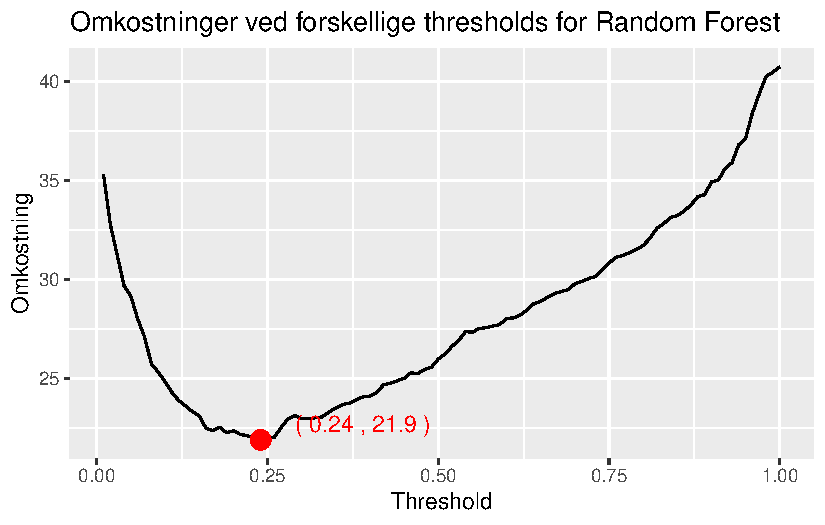
\includegraphics{index_files/figure-pdf/unnamed-chunk-15-1.pdf}

Note that we can find an optimum with a different threshold than 0.50.

Calculates the saved costs of the optimized model (threshold=0.17)
compared to the baseline model (threshold=0.5).''

\begin{Shaded}
\begin{Highlighting}[]
\NormalTok{besparelse\_pr\_kunde }\OtherTok{\textless{}{-}}\NormalTok{ omk\_simple }\SpecialCharTok{{-}} \FunctionTok{min}\NormalTok{(omk)}

\NormalTok{besparelse\_pr\_kunde}\SpecialCharTok{*}\DecValTok{10000}
\end{Highlighting}
\end{Shaded}

\begin{verbatim}
[1] 108254.1
\end{verbatim}

Calculates the saved costs of the optimized model (threshold=0.17)
compared to one's own calculations.''

\begin{Shaded}
\begin{Highlighting}[]
\NormalTok{besparelse\_mavefornemmelse }\OtherTok{\textless{}{-}}\NormalTok{ omkostninger\_mavefornemmelse }\SpecialCharTok{{-}} \FunctionTok{min}\NormalTok{(omk)}

\NormalTok{besparelse\_mavefornemmelse}\SpecialCharTok{*}\DecValTok{10000}
\end{Highlighting}
\end{Shaded}

\begin{verbatim}
[1] 134667.3
\end{verbatim}

We can clearly outperform the existing model that the company uses
(which assumes no churn). We can also clearly outperform the common
50/50 split.

Can we do even better with an alternative model: Let's use linear and
quadratic discriminant analysis and qudratic discriminant analysis, and
we calculate again the total cost savings, and compare them with the
best logistic regression:

\paragraph{Linear Discriminant Analysis
(LDA)}\label{linear-discriminant-analysis-lda}

LDA is a method used for classification and dimensionality reduction. It
finds the best linear combination of features to separate different
classes in the dataset. LDA works well when classes are distinct and
follows normal distributions with equal covariance. It's useful for
understanding which features are most important for classification.
However, it may not perform well with overlapping classes or outliers.
Overall, LDA is effective for classification tasks with well-separated
classes and can provide valuable insights into the data structure.

\begin{Shaded}
\begin{Highlighting}[]
\CommentTok{\# lda}
\NormalTok{lda.fit }\OtherTok{\textless{}{-}} \FunctionTok{lda}\NormalTok{(f, }\AttributeTok{data=}\NormalTok{train)}

\NormalTok{lda.pred }\OtherTok{\textless{}{-}} \FunctionTok{data.frame}\NormalTok{(}\FunctionTok{predict}\NormalTok{(lda.fit, test))}
\NormalTok{omk\_lda }\OtherTok{\textless{}{-}} \FunctionTok{rep}\NormalTok{(}\DecValTok{0}\NormalTok{,}\FunctionTok{length}\NormalTok{(thresh))}
\NormalTok{thresh }\OtherTok{\textless{}{-}} \FunctionTok{seq}\NormalTok{(}\FloatTok{0.01}\NormalTok{, }\FloatTok{1.0}\NormalTok{, }\AttributeTok{length =} \DecValTok{100}\NormalTok{)}

\ControlFlowTok{for}\NormalTok{ (i }\ControlFlowTok{in} \DecValTok{1}\SpecialCharTok{:}\FunctionTok{length}\NormalTok{(thresh)) \{}
\NormalTok{  glm.pred }\OtherTok{\textless{}{-}} \FunctionTok{rep}\NormalTok{(}\StringTok{"No"}\NormalTok{, }\FunctionTok{length}\NormalTok{(lda.pred}\SpecialCharTok{$}\NormalTok{posterior.Yes))  }\CommentTok{\# laver en vektor med No}
\NormalTok{  glm.pred[lda.pred}\SpecialCharTok{$}\NormalTok{posterior.Yes }\SpecialCharTok{\textgreater{}}\NormalTok{ thresh[i]] }\OtherTok{\textless{}{-}} \StringTok{"Yes"} \CommentTok{\# ændrer værdien af glm.pred, hvis p \textgreater{} thresh}
\NormalTok{  glm.pred }\OtherTok{\textless{}{-}} \FunctionTok{as.factor}\NormalTok{(glm.pred) }\CommentTok{\# sikrer, at variablen er en faktor}
\NormalTok{  x }\OtherTok{\textless{}{-}} \FunctionTok{confusionMatrix}\NormalTok{(glm.pred, test}\SpecialCharTok{$}\NormalTok{Churn, }\AttributeTok{positive =} \StringTok{"Yes"}\NormalTok{)}
\NormalTok{  total }\OtherTok{\textless{}{-}}\NormalTok{ x}\SpecialCharTok{$}\NormalTok{table[}\DecValTok{1}\NormalTok{] }\SpecialCharTok{+}\NormalTok{ x}\SpecialCharTok{$}\NormalTok{table[}\DecValTok{2}\NormalTok{] }\SpecialCharTok{+}\NormalTok{ x}\SpecialCharTok{$}\NormalTok{table[}\DecValTok{3}\NormalTok{] }\SpecialCharTok{+}\NormalTok{ x}\SpecialCharTok{$}\NormalTok{table[}\DecValTok{4}\NormalTok{]}
\NormalTok{  TN }\OtherTok{\textless{}{-}}\NormalTok{ x}\SpecialCharTok{$}\NormalTok{table[}\DecValTok{1}\NormalTok{]}\SpecialCharTok{/}\NormalTok{total}
\NormalTok{  FP }\OtherTok{\textless{}{-}}\NormalTok{ x}\SpecialCharTok{$}\NormalTok{table[}\DecValTok{2}\NormalTok{]}\SpecialCharTok{/}\NormalTok{total}
\NormalTok{  FN }\OtherTok{\textless{}{-}}\NormalTok{ x}\SpecialCharTok{$}\NormalTok{table[}\DecValTok{3}\NormalTok{]}\SpecialCharTok{/}\NormalTok{total}
\NormalTok{  TP }\OtherTok{\textless{}{-}}\NormalTok{ x}\SpecialCharTok{$}\NormalTok{table[}\DecValTok{4}\NormalTok{]}\SpecialCharTok{/}\NormalTok{total}
\NormalTok{  omk\_lda[i] }\OtherTok{\textless{}{-}}\NormalTok{ FN}\SpecialCharTok{*}\NormalTok{FN\_omk }\SpecialCharTok{+}\NormalTok{ TP}\SpecialCharTok{*}\NormalTok{TP\_omk }\SpecialCharTok{+}\NormalTok{ FP}\SpecialCharTok{*}\NormalTok{FP\_omk }\SpecialCharTok{+}\NormalTok{ TN}\SpecialCharTok{*}\DecValTok{0}
  
\NormalTok{\}}
\end{Highlighting}
\end{Shaded}

After running the LDA analysis we can compare the savings to the prior
models

\begin{Shaded}
\begin{Highlighting}[]
\CommentTok{\#LDA analysis minimum costs minus logistic analysis minimum costs }
\DecValTok{10000}\SpecialCharTok{*}\NormalTok{(}\FunctionTok{min}\NormalTok{(omk\_lda) }\SpecialCharTok{{-}} \FunctionTok{min}\NormalTok{(omk)) }
\end{Highlighting}
\end{Shaded}

\begin{verbatim}
[1] -400.2001
\end{verbatim}

\begin{Shaded}
\begin{Highlighting}[]
\CommentTok{\#LDA analysis minimum costs minus simple model minimum costs }
\DecValTok{10000}\SpecialCharTok{*}\NormalTok{(}\FunctionTok{min}\NormalTok{(omk\_lda) }\SpecialCharTok{{-}}\NormalTok{ omk\_simple)}
\end{Highlighting}
\end{Shaded}

\begin{verbatim}
[1] -108654.3
\end{verbatim}

\begin{Shaded}
\begin{Highlighting}[]
\CommentTok{\#LDA analysis minimum costs minus own calculation costs}
\DecValTok{10000}\SpecialCharTok{*}\NormalTok{(}\FunctionTok{min}\NormalTok{(omk\_lda) }\SpecialCharTok{{-}}\NormalTok{ omkostninger\_mavefornemmelse)}
\end{Highlighting}
\end{Shaded}

\begin{verbatim}
[1] -135067.5
\end{verbatim}

\paragraph{Quadratic Discriminant Analysis
(QDA)}\label{quadratic-discriminant-analysis-qda}

QDA is similar to LDA but allows for different covariance matrices for
each class, making it more flexible in capturing complex relationships
between features. It works by estimating separate covariance matrices
for each class, which can better capture non-linear decision boundaries.
QDA is beneficial when classes have different variances or when the
decision boundary is non-linear. However, it requires more parameters to
estimate compared to LDA and may overfit with small datasets. Overall,
QDA is useful for classification tasks with non-linear decision
boundaries and varying variances between classes.

\begin{Shaded}
\begin{Highlighting}[]
\CommentTok{\#qda}

\NormalTok{qda.fit }\OtherTok{\textless{}{-}} \FunctionTok{qda}\NormalTok{(f, }\AttributeTok{data=}\NormalTok{train)}
\NormalTok{qda.pred }\OtherTok{\textless{}{-}} \FunctionTok{data.frame}\NormalTok{(}\FunctionTok{predict}\NormalTok{(qda.fit, test))}
\NormalTok{omk\_qda }\OtherTok{\textless{}{-}} \FunctionTok{rep}\NormalTok{(}\DecValTok{0}\NormalTok{,}\FunctionTok{length}\NormalTok{(thresh))}
\NormalTok{thresh }\OtherTok{\textless{}{-}} \FunctionTok{seq}\NormalTok{(}\FloatTok{0.01}\NormalTok{, }\FloatTok{1.0}\NormalTok{, }\AttributeTok{length =} \DecValTok{100}\NormalTok{)}

\ControlFlowTok{for}\NormalTok{ (i }\ControlFlowTok{in} \DecValTok{1}\SpecialCharTok{:}\FunctionTok{length}\NormalTok{(thresh)) \{}
\NormalTok{  glm.pred }\OtherTok{\textless{}{-}} \FunctionTok{rep}\NormalTok{(}\StringTok{"No"}\NormalTok{, }\FunctionTok{length}\NormalTok{(qda.pred}\SpecialCharTok{$}\NormalTok{posterior.Yes))  }\CommentTok{\# laver en vektor med No}
\NormalTok{  glm.pred[qda.pred}\SpecialCharTok{$}\NormalTok{posterior.Yes }\SpecialCharTok{\textgreater{}}\NormalTok{ thresh[i]] }\OtherTok{\textless{}{-}} \StringTok{"Yes"} \CommentTok{\# ændrer værdien af glm{-}pred, hvis p \textgreater{} thresh}
\NormalTok{  glm.pred }\OtherTok{\textless{}{-}} \FunctionTok{as.factor}\NormalTok{(glm.pred) }\CommentTok{\# sikrer at variablen er en faktor}
\NormalTok{  x }\OtherTok{\textless{}{-}} \FunctionTok{confusionMatrix}\NormalTok{(glm.pred, test}\SpecialCharTok{$}\NormalTok{Churn, }\AttributeTok{positive =} \StringTok{"Yes"}\NormalTok{)}
\NormalTok{  total }\OtherTok{\textless{}{-}}\NormalTok{ x}\SpecialCharTok{$}\NormalTok{table[}\DecValTok{1}\NormalTok{] }\SpecialCharTok{+}\NormalTok{ x}\SpecialCharTok{$}\NormalTok{table[}\DecValTok{2}\NormalTok{] }\SpecialCharTok{+}\NormalTok{ x}\SpecialCharTok{$}\NormalTok{table[}\DecValTok{3}\NormalTok{] }\SpecialCharTok{+}\NormalTok{ x}\SpecialCharTok{$}\NormalTok{table[}\DecValTok{4}\NormalTok{]}
\NormalTok{  TN }\OtherTok{\textless{}{-}}\NormalTok{ x}\SpecialCharTok{$}\NormalTok{table[}\DecValTok{1}\NormalTok{]}\SpecialCharTok{/}\NormalTok{total}
\NormalTok{  FP }\OtherTok{\textless{}{-}}\NormalTok{ x}\SpecialCharTok{$}\NormalTok{table[}\DecValTok{2}\NormalTok{]}\SpecialCharTok{/}\NormalTok{total}
\NormalTok{  FN }\OtherTok{\textless{}{-}}\NormalTok{ x}\SpecialCharTok{$}\NormalTok{table[}\DecValTok{3}\NormalTok{]}\SpecialCharTok{/}\NormalTok{total}
\NormalTok{  TP }\OtherTok{\textless{}{-}}\NormalTok{ x}\SpecialCharTok{$}\NormalTok{table[}\DecValTok{4}\NormalTok{]}\SpecialCharTok{/}\NormalTok{total}
\NormalTok{  omk\_qda[i] }\OtherTok{\textless{}{-}}\NormalTok{ FN}\SpecialCharTok{*}\NormalTok{FN\_omk }\SpecialCharTok{+}\NormalTok{ TP}\SpecialCharTok{*}\NormalTok{TP\_omk }\SpecialCharTok{+}\NormalTok{ FP}\SpecialCharTok{*}\NormalTok{FP\_omk }\SpecialCharTok{+}\NormalTok{ TN}\SpecialCharTok{*}\DecValTok{0}
  
\NormalTok{\}}
\end{Highlighting}
\end{Shaded}

After running the QDA analysis we can compare the savings to the prior
models

\begin{Shaded}
\begin{Highlighting}[]
\CommentTok{\#QDA analysis minimum costs minus logistic analysis minimum costs}
\DecValTok{10000}\SpecialCharTok{*}\NormalTok{(}\FunctionTok{min}\NormalTok{(omk\_qda) }\SpecialCharTok{{-}} \FunctionTok{min}\NormalTok{(omk)) }
\end{Highlighting}
\end{Shaded}

\begin{verbatim}
[1] 15007.5
\end{verbatim}

\begin{Shaded}
\begin{Highlighting}[]
\CommentTok{\#QDA analysis minimum costs minus LDA minimums costs}
\DecValTok{10000}\SpecialCharTok{*}\NormalTok{(}\FunctionTok{min}\NormalTok{(omk\_qda) }\SpecialCharTok{{-}} \FunctionTok{min}\NormalTok{(omk\_lda)) }
\end{Highlighting}
\end{Shaded}

\begin{verbatim}
[1] 15407.7
\end{verbatim}

\begin{Shaded}
\begin{Highlighting}[]
\CommentTok{\#QDA analysis minimum costs minus simple model minimum costs}
\DecValTok{10000}\SpecialCharTok{*}\NormalTok{(}\FunctionTok{min}\NormalTok{(omk\_qda) }\SpecialCharTok{{-}}\NormalTok{ omk\_simple)}
\end{Highlighting}
\end{Shaded}

\begin{verbatim}
[1] -93246.62
\end{verbatim}

\begin{Shaded}
\begin{Highlighting}[]
\CommentTok{\#QDA analysis minimum costs minus own calculation costs}
\DecValTok{10000}\SpecialCharTok{*}\NormalTok{(}\FunctionTok{min}\NormalTok{(omk\_qda) }\SpecialCharTok{{-}}\NormalTok{ omkostninger\_mavefornemmelse)}
\end{Highlighting}
\end{Shaded}

\begin{verbatim}
[1] -119659.8
\end{verbatim}

\subsection{Evaluation}\label{evaluation}

We can now asses the performance of the models. As we can see we are
able to save money by focusing on data driven decisions.

\subsection{Deployment}\label{deployment}

The code is scalable since it can be adapted to changes in costs. If we
assume that retention cost is double, we only have to change one
parameter.

\begin{Shaded}
\begin{Highlighting}[]
\NormalTok{TP\_omk }\OtherTok{\textless{}{-}} \DecValTok{80}
\end{Highlighting}
\end{Shaded}

And run the code again.

Furthermore once models are trained and evaluated, they're deployed for
real-world use. Here's how:

\begin{enumerate}
\def\labelenumi{\arabic{enumi}.}
\item
  \textbf{Packaging}: Bundle the trained model with preprocessing steps
  for easy deployment.
\item
  \textbf{Integration}: Integrate the model into existing systems,
  ensuring compatibility.
\item
  \textbf{Optimization}: Optimize for scalability and performance to
  handle real-time requests.
\item
  \textbf{Monitoring}: Monitor model performance over time and update
  regularly.
\item
  \textbf{Security}: Ensure compliance with security regulations and
  protect data privacy.
\item
  \textbf{Documentation}: Provide user-friendly documentation and
  support resources.
\item
  \textbf{Feedback}: Gather feedback for continuous improvement and
  iteration.
\end{enumerate}

\section{Conslusion}\label{conslusion}

Based on the analysis, it is recommended that the bank focuses its
retention efforts on customers identified as high-risk churners by the
predictive models. This targeted approach can help optimize resource
allocation and improve overall customer retention strategies.

In conclusion, the analysis highlights the importance of leveraging
data-driven approaches to understand and address customer churn
effectively. By implementing the recommended strategies, the bank can
enhance customer satisfaction, reduce churn rates, and ultimately, drive
long-term business growth and profitability.



\end{document}
